\documentclass[11pt]{article}
\usepackage[a4paper,margin=2.5cm]{geometry}
\usepackage{amsmath,amssymb,amsthm,booktabs,enumitem,graphicx,hyperref,microtype}
\hypersetup{colorlinks=true,linkcolor=blue,citecolor=blue,urlcolor=blue}
\newtheorem{proposition}{Proposition}
\newtheorem{definition}{Definition}
\newtheorem{corollary}{Corollary}
\title{Temporal Descent from an Atemporal Morphological Body\\
\large Tau Core Foundation Paper V: First Proof Packet}
\author{Jozsef Olcsak}
\date{August 2026}

\begin{document}
\maketitle

\begin{abstract}
This preparation paper isolates the first finite temporal-descent problem in
Tau Core. A stabilized morphological body is not assumed to evolve in an
external parent time. An observer--source resolution map first supplies stable
readout classes; a directed causal quotient may then order those classes. We
prove that order alone cannot determine duration, clock rate, temporal unit or
observer-dependent distortion. We also prove the exact positive-cochain
criterion under which a resolved causal graph admits a path-independent clock,
and give the compatibility condition for two observer clocks on shared
resolved structure. These are conditional internal theorems. Nature has not
yet been proved to select the required positive exact clock form, its absolute
unit, the relativistic limit or a nonzero Tau-specific clock correction.
\end{abstract}

\section{Question and scope}

The paper owns one map:
\begin{equation}
 M_\tau\xrightarrow{\operatorname{Desc}_O}
 \{\text{causal order},t_O,\text{clock rate},\text{temporal resolution}\}.
 \label{eq:target}
\end{equation}
It does not use a temporal process to construct the seed, base or body. The
input is a selected, or explicitly conditional, stabilized body packet. The
observer is embedded in the readout architecture and does not stand outside
the universe.

The present result does not derive physical time from the minimal Tau skeleton,
recover general relativity, predict the age of the universe, or establish an
observer-dependent time anomaly. Its purpose is narrower: determine exactly
what causal order supplies, what it cannot supply, and the minimum additional
source object that turns order into a clock.

\begin{figure}[t]
 \centering
 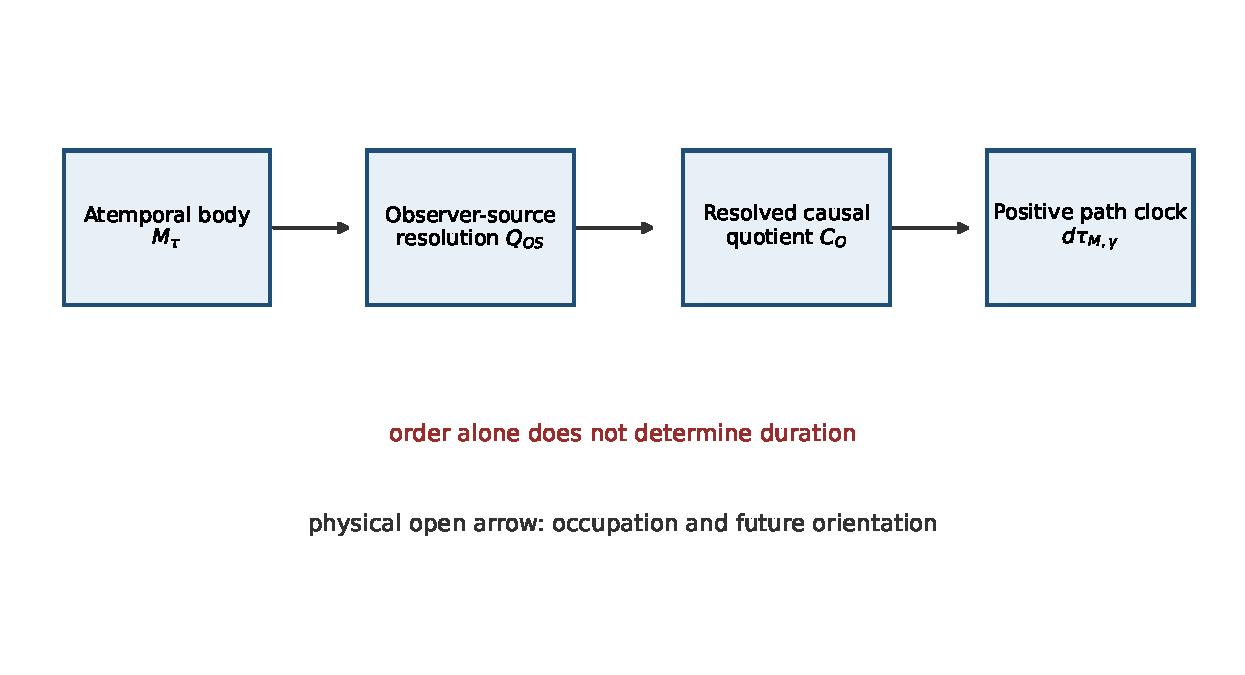
\includegraphics[width=.94\linewidth]{figures/fig_temporal_descent_spine.pdf}
 \caption{The first temporal-descent spine. The observer-relative stable
 partition is part of the operational quantization; causal order alone does
 not fix duration. The open physical arrow selects the positive exact clock
 form.}
 \label{fig:spine}
\end{figure}

\section{Stable observer-relative resolution}

Let \(X_{OS}\) denote the body-conditioned observer--source configuration
domain. A finite-resolution readout is a stable map
\begin{equation}
 Q_{OS}:X_{OS}\longrightarrow \mathcal E_O,
\end{equation}
and two configurations are operationally equivalent when
\begin{equation}
 x\sim_O y \quad\Longleftrightarrow\quad Q_{OS}(x)=Q_{OS}(y).
 \label{eq:equivalence}
\end{equation}
This equality, not a bare condition of the form \(d(x,y)<\epsilon\), defines
the observer-relative readout classes. A threshold-neighbour relation need not
be transitive and therefore does not by itself define a quotient.

The resolved classes inherit a directed relation \(\prec_O\) only when the
body-conditioned full readout annihilates the declared nulls and preserves the
parent orientation on the quotient. We write the resulting finite directed
acyclic graph as \(C_O=(\mathcal E_O,E_O)\). Its acyclicity is an assumption of
this first packet, not a theorem about every possible parent completion.

\section{Order-only no-go}

\begin{proposition}[Order-only no-go]
Suppose a real-valued label \(t:\mathcal E_O\to\mathbb R\) is strictly
increasing on every edge of \(C_O\). Then every strictly increasing function
\(f\) produces the equally order-compatible label \(f\circ t\). Consequently
the directed order alone determines neither elapsed duration, clock rate,
clock unit nor observer-dependent time distortion.
\end{proposition}

\begin{proof}
For every directed edge \(u\to v\), strict monotonicity gives
\(t(u)<t(v)\). Since \(f\) is strictly increasing,
\(f(t(u))<f(t(v))\). The complete order is therefore unchanged while finite
differences and their ratios can change. In particular
\(t\mapsto at+b\), \(a>0\), leaves order invariant and changes the unit and
origin.
\end{proof}

This no-go separates temporal orientation from metric time. It also blocks a
common overclaim: an oriented causal incidence is not by itself a physical
clock.

\section{Exact positive clock form}

\begin{definition}[Observer clock form]
An observer clock form is a positive edge cochain
\begin{equation}
 \tau_O:E_O\longrightarrow\mathbb R_{>0}.
\end{equation}
It is exact when there exists \(t_O:\mathcal E_O\to\mathbb R\) such that
\begin{equation}
 \tau_O(u,v)=t_O(v)-t_O(u)
 \label{eq:exact}
\end{equation}
for every directed edge \(u\to v\).
\end{definition}

\begin{proposition}[Exact-clock criterion]
On a connected finite resolved causal graph, a positive edge cochain defines a
path-independent observer clock if and only if its sums agree on every pair of
directed paths with common endpoints. Equivalently, its circulation vanishes
on every cycle in the undirected cycle space. With \(\tau_O\) fixed, the clock
is unique up to one additive constant.
\end{proposition}

\begin{proof}
If Eq.~\eqref{eq:exact} holds, summing along a path telescopes to the endpoint
difference, so all paths agree. Conversely choose a reference event \(e_0\)
and define \(t_O(e)\) as the sum of \(\tau_O\) along any path from \(e_0\) to
\(e\), reversing signs for oppositely traversed edges. The zero-circulation
condition makes this definition path independent and yields
Eq.~\eqref{eq:exact}. Two potentials with the same edge differences differ by
a constant on a connected graph.
\end{proof}

If the source fixes only the ray \([\tau_O]\), a positive scale freedom remains
and clocks are unique only up to \(t_O\mapsto at_O+b\), \(a>0\). Thus the clock
form and its absolute unit are distinct physical obligations.

\begin{figure}[t]
 \centering
 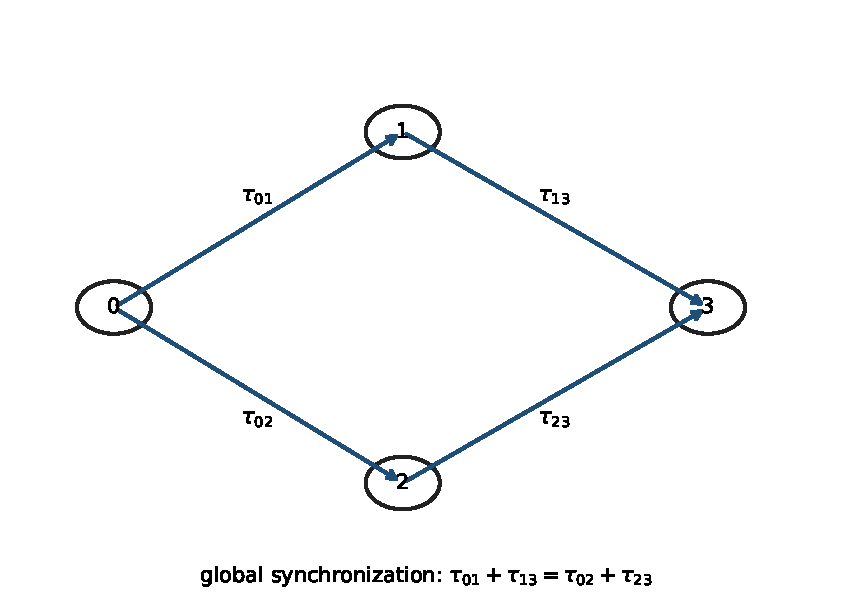
\includegraphics[width=.66\linewidth]{figures/fig_clock_diamond.pdf}
 \caption{The minimal path-independence audit. A causal diamond admits one
 endpoint clock difference exactly when the two path sums agree.}
 \label{fig:diamond}
\end{figure}

\begin{corollary}[Diamond condition]
For the graph in Fig.~\ref{fig:diamond}, a clock exists exactly when
\begin{equation}
 \tau_{01}+\tau_{13}=\tau_{02}+\tau_{23}.
 \label{eq:diamond}
\end{equation}
The difference of the two sides is clock holonomy and cannot be discarded as
gauge if a terminal can observe it.
\end{corollary}

\section{Compatibility of different observers}

Different observers may resolve different partitions and assign different
rates without logical contradiction. Let a shared refinement \(C_{12}\) map
to the two observer quotients by \(r_i:C_{12}\to C_i\).

\begin{proposition}[Shared-clock compatibility]
Two observer clocks preserve one common temporal orientation on their shared
resolved domain when their pulled-back edge forms are positive and satisfy
\begin{equation}
 r_1^*\tau_1=\lambda_{12}\,r_2^*\tau_2,
 \qquad \lambda_{12}>0,
 \label{eq:observer-compatibility}
\end{equation}
on each connected comparison component. They then disagree at most by a
positive rate and an additive origin. A negative factor reverses orientation;
non-proportional forms encode genuine observer-dependent clock response rather
than a mere change of units.
\end{proposition}

The proposition does not require all observers to occupy the same body event.
It requires their overlapping readouts to preserve the source orientation.
Observer dependence therefore changes accessible information, resolution and
possibly clock rate without granting arbitrary contradictory causal arrows.

\section{Paper-IV discriminator interface}

Paper IV freezes the three-readout vector
\begin{equation}
 \delta Y=(\delta\rho,\delta p\ \text{or}\ \delta\Pi,\delta T)^{\mathsf T}
\end{equation}
and a primary-null determinant \(Z_\tau=\det[a\ b\ \delta Y]\). In this paper
the final component is not an independently fitted time residual. Once
\(\tau_O\) is source-derived, it is defined by the linearized response
\begin{equation}
 \delta T= D_s t_O[\delta s]
 \label{eq:clock-row}
\end{equation}
under the same frozen morphology descriptor and observer quantizer. Until
Eq.~\eqref{eq:clock-row} is derived and the standard clock response is
controlled, the Paper-IV contrast is a protocol handoff rather than a physical
Tau prediction.

\section{What is proved and what remains open}

The finite result is now sharp:
\begin{center}
\begin{tabular}{p{.44\linewidth}p{.42\linewidth}}
\toprule
Result & Status\\
\midrule
Stable \(Q_{OS}\) defines observer-relative readout classes & definition\\
Order alone fixes duration or rate & disproved\\
Positive exact edge form defines a clock & proved\\
Fixed clock form gives uniqueness up to origin & proved\\
Clock-form ray gives uniqueness up to positive affine change & proved\\
Shared observer compatibility criterion & proved conditionally\\
Physical parent selects \(\tau_O\) and its unit & open\\
Standard relativistic limit and nonzero Tau excess & open\\
\bottomrule
\end{tabular}
\end{center}

The next bounded proof task is not another ordering gate. It is to test the
existing selected body packet for a source-owned positive one-form whose
descent is exact on the observer quotient and whose local limit equals proper
time. Failure has a finite verdict: either the packet lacks physical clock
content, or the relevant nonzero holonomy must be retained as a new observable
instead of being quotiented away.

\section{Conclusion}

An atemporal morphological body can contain a temporal readout without first
being placed in an external time. Stable observer-relative quantization gives
resolved events; inherited orientation orders them; a positive exact clock
form assigns durations. The first two ingredients do not imply the third. This
paper therefore converts the temporal-descent problem into one concrete source
question: does the selected physical body packet supply and occupy the exact
positive form whose observer descent recovers proper time and fixes the clock
row used by downstream multi-readout tests? The mathematical criterion is
closed; physical source selection remains open.

\end{document}
